\chapter {Różnica symetryczna jako sposób porównywania odcisków}

Większość obecnie stosowanych metod porównuje odciski poprzez szukanie podobieństw między nimi. Metody nie zastanawiają się nad wpływem ilości niepodobnych minucji. Celem tej pracy jest stwierdzenie czy istnieje możliwość porównywania odcisków badając jedynie ich niepodobieństwo. Sposób ten stara się odpowiedzieć na pytanie co jest lepsze 10 zgodnych minucji, które stanowią jedynie 33\% wszystkich minucji, czy wzorca, czy 4 zgodne minucje które stanowią 50\% minucji wzorca. W obecnie stosowanych standardach liczba cech wspólnych wymaganych przez prawo lub procedury kryminalistyczne do ustalenia tożsamości wynosi\footnote{dane zaczerpnięte ze strony http://pl.wikipedia.org/wiki/Linie\_papilarne}
\renewcommand*{\labelitemi}{\bullet}
\begin{itemize}
	\item 8-12 Niemcy
	\item 17 Francja
	\item 15 Polska
\end{itemize}
\vspace{.5cm}\par
A w przypadku minucji rzadziej występujących liczba ich może być nawet mniejsza. Natomiast nigdzie nie doszukano się maksymalnych liczb niezgodnych minucji. Jedyne dodatkowe ograniczenia wprowadzają same SDK'i. Przykładowo SDK $Neurotechnology$ w standardowej konfiguracji przyjmuje minimalną liczbę minucji jako 10. Nie jest to jednak, żadna arbitralnie wyznaczana przez prawo wartość, a jej wartość można ustalać według własnych preferencji. Powstało założenie, że liczba minucji niezgodnych powinna być większa dla porównań między różnymi odciskami. Metoda podobnie jak sprawdzanie podobieństwa wrażliwa jest na liczbę minucji w porównywanych odciskach. Dlatego warto uzyskaną liczbę niezgodność podzielić przez ilość minucji w odciskach. Nie stosuje się oddzielnych statystyk dla niezgodności porównań 1:0 i 0:1. Statystyki te to nic innego jak porównywania przedstawione w rozdziale 4. Istnieje liniowa zależność między porównaniami co prezentuje wzór \ref{eq:dependency}.

\begin{equation}
Q_s = \frac{C_{1-1}}{C_{pattern}}
\label{eq:Q_s}
\end{equation}

\begin{equation}
Q_{ns} = \frac{C_{1-0}}{C_{pattern}}
\label{eq:Q_ns}
\end{equation}

\begin{equation}
Q_s = 1 - Q_{ns} 
\label{eq:dependency}
\end{equation}

\begin{table}
\begin{tabular}{l l p{13cm}}
\bullet & Q_s &  Jakość kodu(procent zgodności) \\
\bullet & Q_{ns} & Jakość kodu(procent niezgodności)\\
\bullet & C_{1-1} & Ilość porównań 1:1 dla \\
\bullet & C_{1-0} & Ilość porównań 1:0 \\
\bullet & C_{pattern} & Ilość minucji we wzorcu\\
\end{tabular}
\end{table}

\section[Analiza statystyczna kodu][Analiza statystyczna kodu]{Analiza statystyczna kodu}
Zastosowane rozwiązanie wylicza jakość niedopasowania jako iloraz sumy ilości porównań 1:0 i 0:1 do sumy ilości minucji wzorca i rozpatrywanych minucji próbki. Rozwiązanie przedstawia wzór\ref{eq:Q_nss}

\begin{equation}
Q_nss = 1 - \frac{C_{1-1}}{(C_{pattern} + C_{sample})}
\label{eq:Q_nss}
\end{equation}

\begin{table}
\begin{tabular}{l l p{13cm}}
\bullet & Q_{nss} & Jakość kodu(procent niezgodności) dla różnicy symetrycznej\\
\bullet & C_{sample} & Ilość rozpatrywanych minucji w próbce\\
\end{tabular}
\end{table}

W odróżnieniu od poprzedniego jest liniowo niezależny od jakości kodu przedstawianych w rozdziale 4. Gdyby tak nie było zabieg taki nie miałby większego sensu. Podobnie jak w poprzednim rozdziale świadomie zastąpiono odległości Hamminga porównując jedynie charakterystyczne porównania. Zbędne tło (porównania 0:0) jest pomijane. Wyniki z komercyjnego oprogramowania przedstawiane są jako porównanie. Podobnie jak wcześniej SDK $Neurotechnology$ użyto jedynie do zdobycia liczby minucji zgodnych i niezgodnych. Liczba porównań jest taka sama jak w poprzednim rozdziale i przeprowadzona została na tej samej próbie odcisków.

\subsection{Rezultaty testów}
Kolorem czerwonym zaznaczono porównania między odciskami pochodzącymi od różnych palców, zielonym pochodzących od tych samych. Przedstawione wyniki również nie są wystarczajaco dobre, natomiast są nieco lepsze niż w przypadku porównywania podobieństwa. EER zmniejszył się i wynosi ok 17\%. Nie jest to wynik zadowalający ale warto zauważyć, że zmieniono jedynie sposób porównania a nie sam algorytm kodowania. Każda poprawa wyniku jest więc sukcesem. FAR dla ustalonego progu wynosi ok 13\% i w porównaniu do poprzedniej metody uległ niewielkiemu pogorszeniu( 2 punkty procentowe). FRR wynosi ok 18\% i uległo sporej poprawie względem poprzedniej metody (5 punktów procentowych). Błędy ZERO FAR i ZERO FRR dalej są na poziomie niedopuszczalnym i wynoszą ponad 95\%. Kolejnym ciekawym zjawiskiem jest zwężenie przedziałów w jakich znajdują się wykresy. Niestety zmiana ta dotyczy zarówno porównań różnych jak i tych samych odcisków. Przedstawiona symulacja dowodzi iż sposoby porównywania niezgodności lepiej sprawdza się dla porównywania odcisków pochodzących od jednego palca. Natomiast sposób porównywania zgodności lepiej sprawdza się dla porównywania odcisków pochodzących od różnych palców. Wynik jest zaskakujący gdyż działa inaczej niż wskazywałoby na to logiczne rozumowanie. 

\subsubsection{Teza 1}
Stwierdzanie podobieństwa jest skuteczniejsze poprzez porównywanie niepodobieństw.

\subsubsection{Teza 2}
Stwierdzanie niepodobieństwa jest skuteczniejsze poprzez porównywanie podobieństw.
\vspace{.5cm}\par

Plusem tej metody jest brak konieczności rozstrzygania wyniku dla porównań względem próbki i dla porównań względem wzorca. W poprzedniej metodzie właściwie otrzymywano dwa wskazania w zależności czy liczbę dopasowań podzielono przez liczbę minucji wzorca czy liczbę rozpatrywanych minucji próbki. W tej metodzie wyróżniono tylko jeden współczynnik. Możliwym wyjściem jest stosowanie hybrydy tych dwóch rozwiązań. Zastosować można to dla tych porównań które znajdują się blisko progu decyzyjnego. w takiej sytuacji należało by skorzystać z drugiego wskaźnika i w przypadku przeciwnego rezultatu, wybrać ten który znajduje się dalej od swego progu decyzyjnego. Być może taka hybryda łączyła by mocne strony obu sposobów porównań mogłoby to doprowadzić do kolejnego zmniejszenia błędów dopasowań odcisków. 

\begin{figure}[!htb]
    \begin{center}
		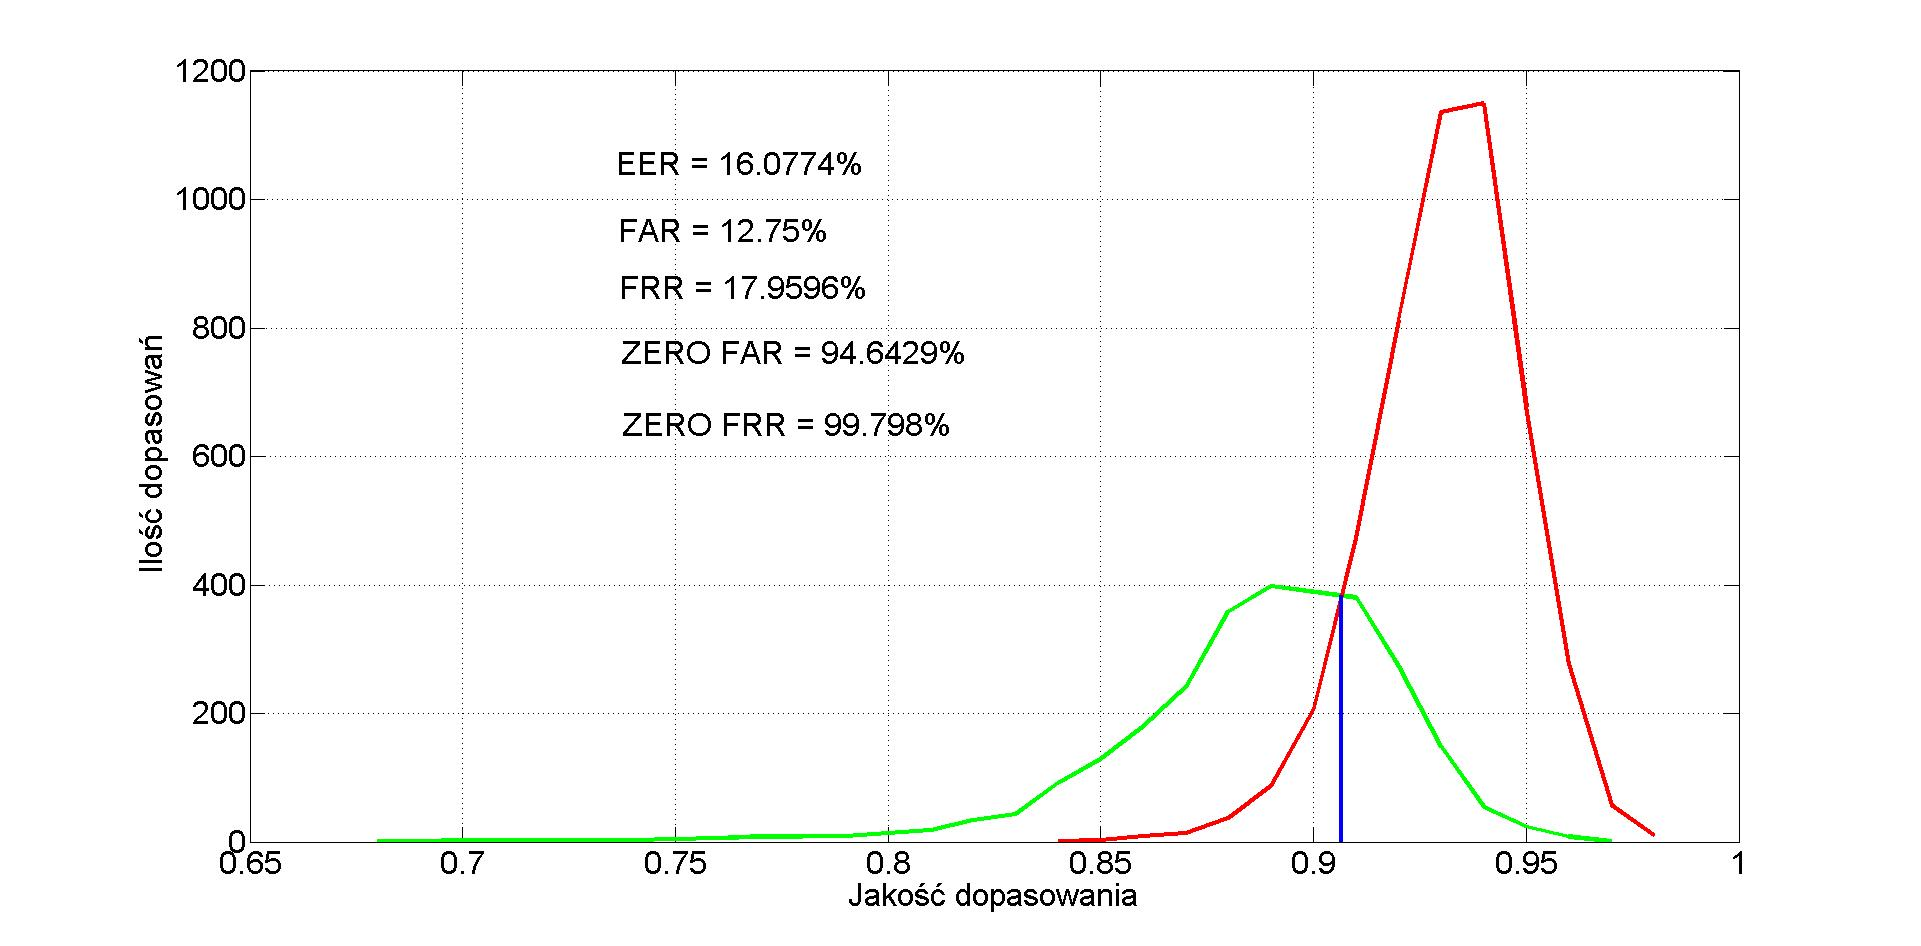
\includegraphics[angle=0,scale=0.27]{img/simetric_distance_code_line.jpg}
		\caption{Ilość niedopasowań w zależności od jakości niedopasowania do odcisków}
		\label{img:code_simetric_line}
    \end{center}
\end{figure} 
Niestety test ten dowodzi iż niezależnie od metody porównywania dla zaproponowanego algorytmu jest nieskuteczne jeśli porównujemy tylko jeden wskaźnik takiego porównania. Niezależnie czy porównujemy podobieństwo czy niepodobieństwo błąd EER jest niedopuszczalny i nie czyni tworzonej metody systemem biometrycznym. Celowo nie sprawdzam hybrydowego rozwiązania gdyż nawet polepszenie wyniku o kilka punktów procentowych nie jest rozwiązaniem. Jedyną drogą rozwiązania problemu jest wykorzystanie wszystkich danych tworzonych przez porównywanie i badanie rozkładu punktów porównań w przestrzeni trójwymiarowej. Metoda oraz jej wyniki opisana jest w rozdziale 6.
\vspace{.5cm}\par

Na wykresie \ref{img:ob_simetric_line} Przedstawiono tą samą metodę wykorzystując SDK $Neurotechnology$ jedynie do zdobycia liczby minucji pasujących i niepasujących. W zastosowaniu algorytmu kodującego, jak również dla listy minucji z SDK'a zaobserwowano poprawę wskaźnika EER i FRR wskaźnik FAR został bez zmian. Ponieważ zmiana zachowań współczynników jest powtarzalna dla podejścia kodowego i obiektowego, dlatego tezy 1 i 2 można uznać za prawdziwe. Plusem tej obserwacji jest to iż postawione tezy nie zależą od stosowanych algorytmów. Podobnie jak w porównywaniu podobieństwa dane zebrane z komercyjnego SDK mają lepsze wyniki od podejścia kodowego. Dowodzi to iż kodowa wersja algorytmu w połączeniu z tymi metodami porównywania odcisków nie jest wystarczająco dobra do poprawnej weryfikacji. 

\begin{figure}[!htb]
    \begin{center}
		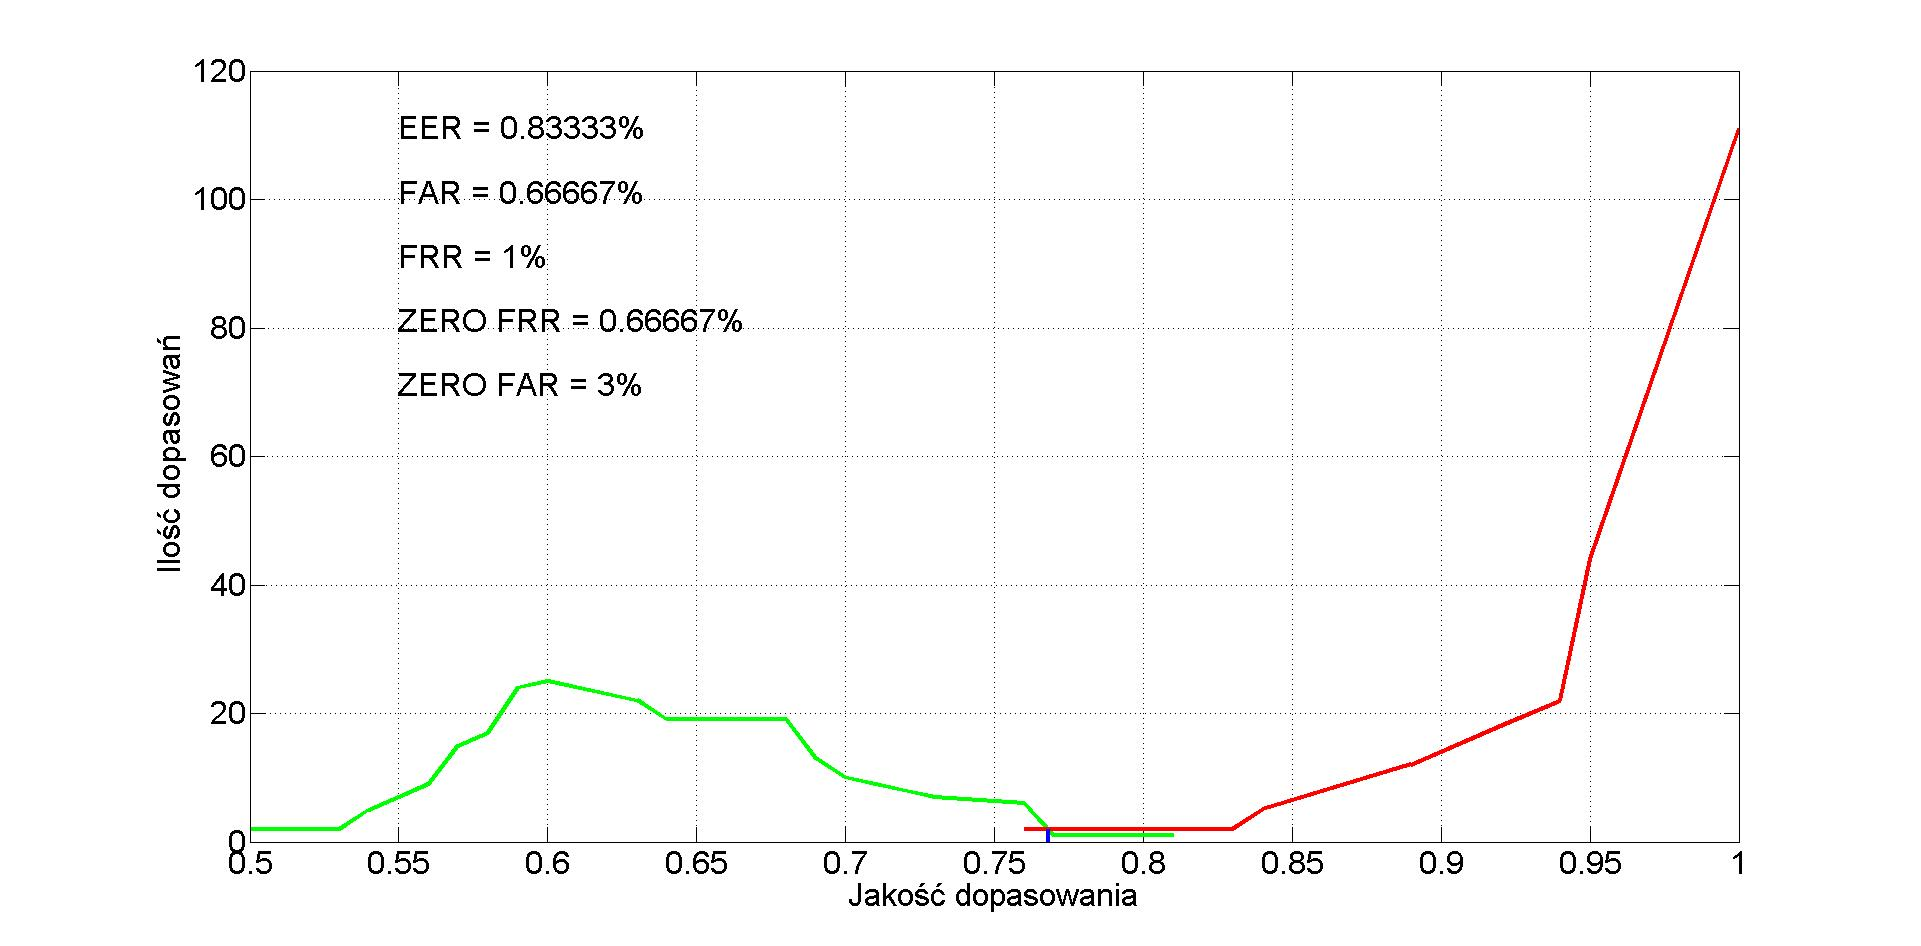
\includegraphics[angle=0,scale=0.27]{img/simetric_distance_ob_line.jpg}
		\caption{Ilość niedopasowań w zależności od jakości niedopasowania do odcisków}
		\label{img:ob_simetric_line}
    \end{center}
\end{figure} 